\section{Testing}
Bash scripts have been written to aid with the testing of the program,
which can be found in the \verb|test| folder. Some of the games are tested
by hand and cross-checked using existing pieces of software, and methods
such as best response diagrams. Amongst the games chosen for the test cases
are identity games (in \verb|test/identity|), $\Gamma(d \times d)$ and 
$\Gamma(d \times 2d)$ dual cyclic polytopes, and some other games.

Most of the automated tests for path and path lengths, have two similar
file names, \verb|*m1| and \verb|*m2| these files run the specified
test using method 1 and method 2 of initialisation for the Lemke's algorithm.

For automated testing of identity matrix games, the size of the game to be tested
is required as an argument of the bash script which runs the test. The script then
generates the game, and the first set of paths from the artificial equilibrium,
and tests to see if the paths generated for the given missing labels, are the same
as the paths computed by the program.

The same method for testing applies to $\Gamma(d\times d)$ dual-cyclic polytope
games, where the paths are generated and checked to see if it is the same 
equivalent path which the program computed. The Maple script provided by Rahul
Savani used to generate
the dual-cyclic polytope games is available at \verb|test/dualcyclic/thesis.mws|.
Some sample games which were generated by the Maple script have also been provided,
and are used in the tests. In addition to testing the paths, another test case was
added to confirm that the equilibrium found by the program was a unique equilibrium.

In testing the $\Gamma(d \times 2d)$ dual-cyclic polytope games, the path length of
the first couple of pivots from the artificial equilibrium was tested using already known
values for the length of the path \cite{rahul}. The paths of the $(2 \times 4)$ game was computed
using the manipulation of bit strings and is also provided 
(\verb|test/dualcyclic/dx2d/2x4bit|).

Other tests were carried out using best response diagrams to find the equilibria
reachable by Lemke-Howson, and compare with the results gotten from the program.
Some of these tests can be found in the figures that are attached below.

The game in Figure \ref{uniqeq} contains exactly one equilibrium, which is
reached from the artificial equilibrium using all the strategies 1 through
6. The game shown in Figure \ref{oneeq} contains three different Nash
Equilibrium, but only one equilibrium the pure strategy 
$
\begin{pmatrix}
    (0 & 0 & 1) &(0 & 0 & 1)
\end{pmatrix}
$
\fbox{
\begin{picture}(0,0)
    \color{blue}\put(0,5){\circle*{7}}
\end{picture}} 
is reachable with the Lemke-Howson algorithm. Finally, the game represented
in Figure \ref{multeq}, has 5 Nash Equilibria all of which can be found
with the Lemke-Howson algorithm. Using the missing labels 1 through 6 from
the artificial equilibrium, we get the following equilibria.
\begin{itemize}
    \item Labels 1 and 4 leads to equilibrium 
        \fbox{
        \begin{picture}(0,0)
            \color{red}\put(0,5){\circle*{7}}
        \end{picture}}
    \item Labels 2 and 5 leads to equilibrium 
        \fbox{
        \begin{picture}(0,0)
            \color{green}\put(0,5){\circle*{7}}
        \end{picture}}
    \item Labels 3 and 6 leads to equilibrium 
        \fbox{
        \begin{picture}(0,0)
            \color{yellow}\put(0,5){\circle*{7}}
        \end{picture}}  
    \item Restarting from equilibrium
        \fbox{
        \begin{picture}(0,0)
            \color{red}\put(0,5){\circle*{7}}
        \end{picture}}
        with labels 2, 3, 5, 6 leads to
        \fbox{
        \begin{picture}(0,0)
            \color{blue}\put(0,5){\circle*{7}}
        \end{picture}}
    \item Restarting from equilibrium
        \fbox{
        \begin{picture}(0,0)
            \color{green}\put(0,5){\circle*{7}}
        \end{picture}}
        with labels 1, 4 leads to
        \fbox{
        \begin{picture}(0,0)
            \color{blue}\put(0,5){\circle*{7}}
        \end{picture}}
    \item Restarting from equilibrium
        \fbox{
        \begin{picture}(0,0)
            \color{green}\put(0,5){\circle*{7}}
        \end{picture}}
        with labels 3, 6 leads to
        \fbox{
        \begin{picture}(0,0)
            \color{purple}\put(0,5){\circle*{7}}
        \end{picture}}
    \item Restarting from equilibrium
        \fbox{
        \begin{picture}(0,0)
            \color{yellow}\put(0,5){\circle*{7}}
        \end{picture}}
        with labels 1, 2, 4, 5 leads to
        \fbox{
        \begin{picture}(0,0)
            \color{purple}\put(0,5){\circle*{7}}
        \end{picture}}
\end{itemize}

\begin{figure}[tbh]
    \caption{$3 \times 3$ Game}\label{uniqeq}
    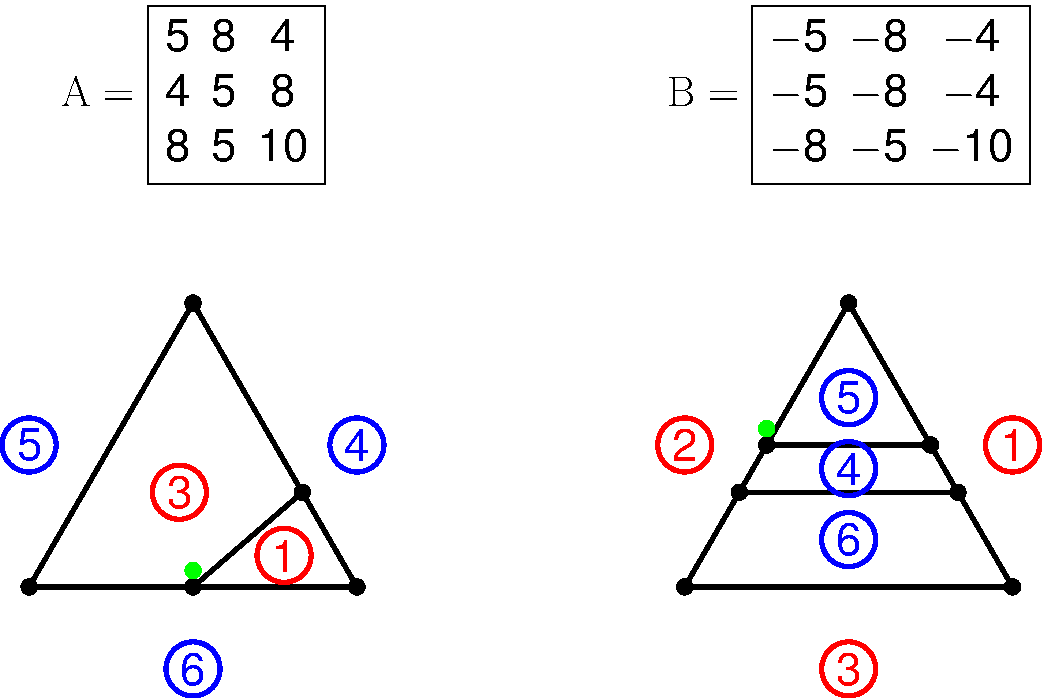
\includegraphics[width=\textwidth]{img/img1.pdf}
\end{figure}

\begin{center}
    \begin{figure}[tbh]
        \caption{$3 \times 3$ Game}\label{oneeq}
        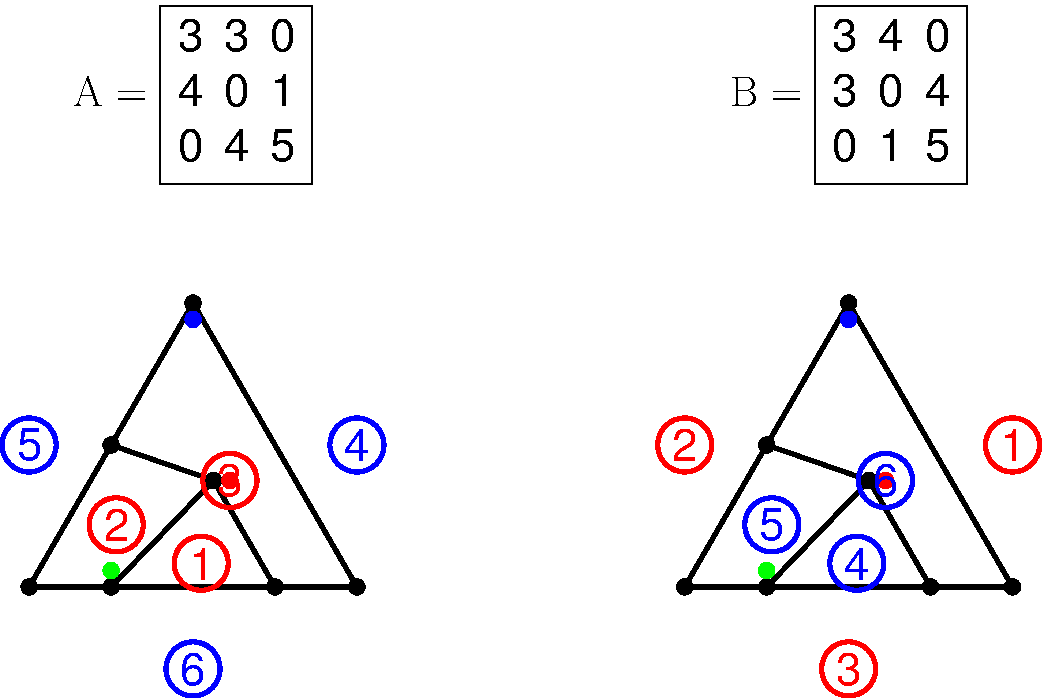
\includegraphics[width=\textwidth]{img/img0.pdf}
    \end{figure}
\end{center}

\begin{figure}[tbh]
    \caption{$3 \times 3$ Game}\label{multeq}
    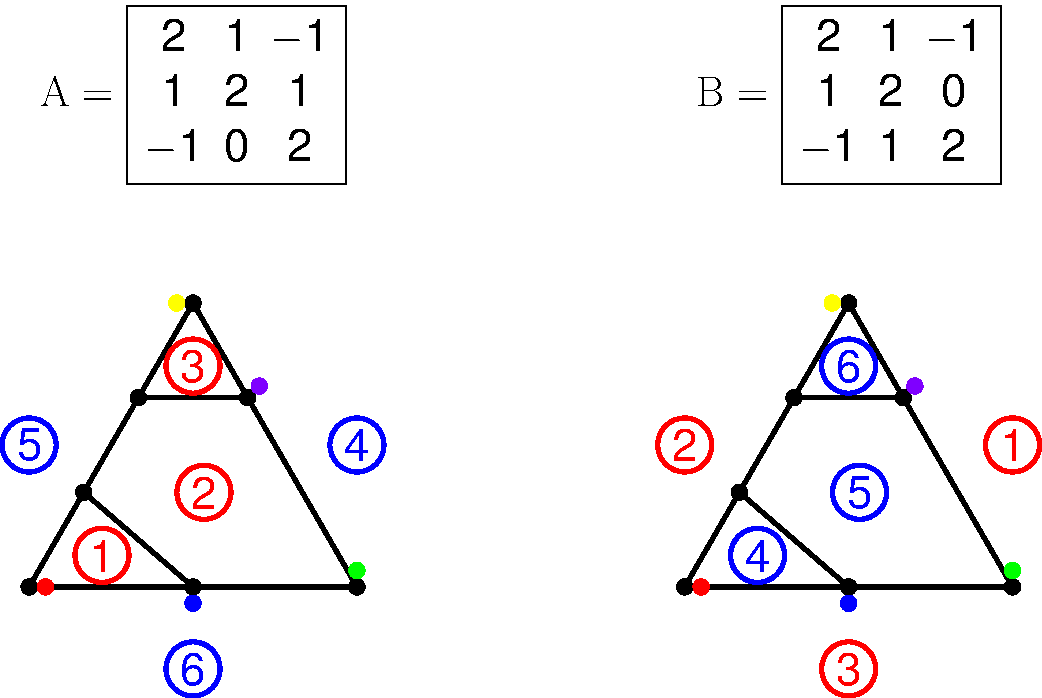
\includegraphics[width=\textwidth]{img/img2.pdf}
\end{figure}
